\documentclass[conference]{IEEEtran}

% Paquets necessaris
\usepackage{graphicx} % Per incloure imatges
\usepackage{courier}
\usepackage[catalan]{babel} % Per usar el català
\usepackage{multicol}
\usepackage{titlesec}
\usepackage{dsfont}
\usepackage{pgffor}
\usepackage{amsfonts}
\usepackage{algorithm}
\usepackage{algpseudocode}
\usepackage[x11names]{xcolor}
\usepackage[colorlinks = true,
            linkcolor = blue,
            urlcolor  = blue,
            citecolor = blue,
            anchorcolor = blue]{hyperref}%hiperenllaços

% Configuración de las columnas
\setlength{\columnsep}{0.2 in} % Separación entre columnas
\setlength{\columnwidth}{3.5 in} % Ancho de cada columna

\titleformat{\subsubsection}
  {\normalfont\bfseries\large}{\thesubsubsection}{1em}{\quad}
\renewcommand\thesubsubsection{\thesubsection.\arabic{subsubsection}}




% Cambiar el formato de numeración de las secciones
\renewcommand{\thesection}{\arabic{section}}
\renewcommand{\thesubsection}{\thesection.\arabic{subsection}}
\newcommand\colorrulemix[1]{\textcolor{#1!40!gray}{\rule{1cm}{1cm}} }
\newcommand\colorrule[1]{\textcolor{#1}{\rule{1cm}{1cm}} }

\titleformat{\section}{\normalfont\Large\bfseries}{\thesection}{1em}{}
\titleformat{\subsection}{\normalfont\large\bfseries}{\thesection.\arabic{subsection}}{1em}{}

\pagestyle{plain}
\pagenumbering{arabic}


% Información del documento
\title{Pràctica 4: Recorregut de camins mínim}
\author{Jaume Adrover Fernandez, Diego Bermejo Cabañas i Joan Balaguer Llagostera}

\begin{document}
\maketitle

\begin{abstract}
    En aquest document s'explicarà el contingut de la pràctica 4 sobre trobar el camí més curt entre dos pobles d'Eivissa i Formentera, passant per un altre obligatòriament. Explicarem com hem afrontat el problema, quines solucions hem implementat,  el codi desenvolupat i finalment unes conclusions amb els problemes que ens hem trobat i algunes reflexions que hem fet.
\end{abstract}

% Introducción
\section{Introducció}
En aquest article explicarem el funcionament i la implementació de la nostra pràctica, estructurant el document de tal forma que es cobreixi la totalitat de aspectes rellevants d'aquesta.\\\\
Per una part explicarem l'estructura del MVC que hem relitzat i mostrarem analíticament com funciona aquesta estructura durant l'execució del programa.\\\\
A continuació, explicarem breument el problema que ens han proposat resoldre. Mostrarem analíticament les dues solucions que hem implementat per resoldre el problema, juntament amb explicacions en pseudocodi perquè posteriorment es pugui entendre millor el codi que hem implementat\\\\
Després, mostrarem el codi implemementat per a resoldre el problema tal i com l'hem explicat a l'apartat anterior.\\\\
Finalment, explicarem com funciona la nostra aplicació una vegada s'executa, a més del problemes que ens hem trobat i com els hem acabat resolguent.\\
\section{Implementació del MVC}
Una estructura MVC (Model Vista Controlador), consta de 3 grans parts: 
\begin{itemize}
  \item \textbf{Model}: és l'encarregat d'emmagatzemar les dades del programa.\\
  \item \textbf{Vista}: s'encarrega de mostrar la interfície d'usuari amb les dades del model.\\
  \item \textbf{Controlador}: encarregat de notificar canvis de la vista entre el programa principal i el model de dades.\\
\end{itemize}
 Una vegada sabem el que simbolitza cada part de l'estructura, podem entrar més en detall en el que fa cada una d'aquestes a la nostra pràctica. Per entendre-ho millor, exemplificarem el paper que jugarà cada una de les parts quan executem el programa.

 \begin{itemize}
    %CANVIAR QUE S'INSTANCIA AQUI EL MAPA
    \item Una vegada es posa en marxa el programa principal, aquest, crear el model de dades i la vista. D'aquesta forma, es mostra al panell la imatge del mapa d'Eivissa i Formentera, sense cap tipus de nodes ni arestes. El controlador s'inicialitza a null, ja que de moment no s'hauran produït canvis a la vista.\\

    \item L'estructura, esdevindrà d'aquesta forma fins al moment en què l'usuari cliqui un dels 3 botons de la finestra (ja que és l'única forma que té d'interactuar amb l'aplicació i que es produeixin canvis a aquesta). A l'hora de clicar un botó, la vista avisa al programa principal, que es la central responsable dels canvis.\\
    
    \item Una vegada el programa principal sap quin dels botons s'ha clicat, aquest se li notificarà i actuarà en conseqüència (els casos específics s'explicaran quan expliquem el programa principal).\\

    \item Quan el programa principal rep la instrucció de lectura de fitxer, aquest s'encarrega d'inserir al model l'estructura d'un graf. Això es fa mitjançant un arxiu \textit{XML}, que conté una enumeració de tots els pobles i les carreteres pertanyents a aquest mapa. Tota aquesta informació es troba a una instància de la classe \textit{Mapa}.\\

    \item A continuació, l'usuari ha de seleccionar 3 pobles diferents, per a poder calcular una ruta entre el primer i el darrer, passant per l'intermedi. Aquest camí sirà el més curt possible. En haver seleccionat els 3 pobles diferents, clicam el botó de calcular.\\
    
    \item El controlador notifica a la classe \textit{Dijkstra}, que ha d'intentar trobar una solució amb les dades que hi ha al model. D'aquesta manera, s'anirà recorrent el graf fins a trobar un vector amb les distàncies mínimes des d'un origen determinat.\\

    
    \item Una vegada acabi l'execució de l'algorisme, les dades del model ja estaran actualitzades i des del Controlador notificarem a la Vista que torni a repintar el panell on es mostra el mapa.\\


    \item Finalment, en cas de voler tornar a calcular una altra ruta des de pobles diferents, clicam el botó de Reset i podrem tornar a seleccionar 3 pobles diferents
\end{itemize}

\begin{figure}[ht]
    \centering
    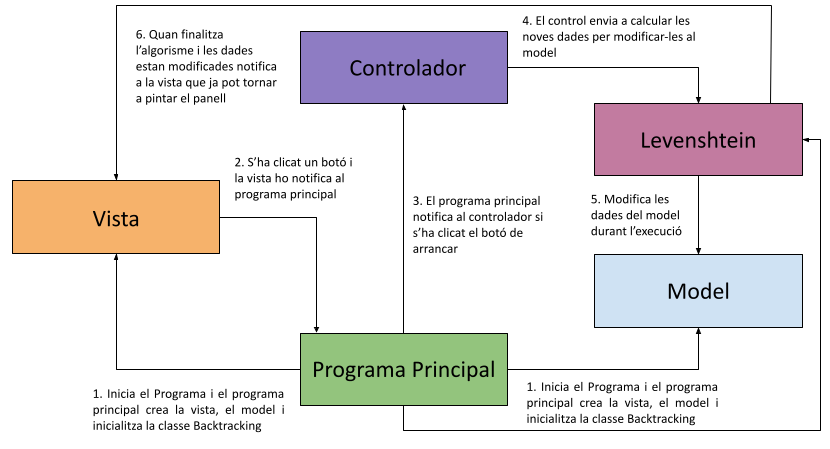
\includegraphics[width=0.388\textwidth]{images/MVC.png}
    \caption{Esquema de com funciona el nostra MVC}
\end{figure}

%3.IMPLEMENTACIÓ DE LA SOLUCIÓ
\section{Implementació de la solució}

\subsection{Problemes a resoldre}
    Durant el desenvolupament d'aquesta pràctica, hem tingut diferents inconvenients/dubtes. Vegeu la llista:

    \begin{itemize}
        \item \textbf{Obtenció del graf}: un dels nostres dubtes principals a l'hora de obtenir el graf era com podíem obtenir tota la informació d'alguna manera eficient.
        \item \textbf{Conversió a estructura adient}: hi ha moltes variacions de l'algoritme Dijkstra però no sabíem quina estructura havíem d'utilitzar per al recorregut d'aquest.
        \item \textbf{Representació visual}: una altra sospita que vàrem tenir va ser a l'hora de representar visualment el camí, ja que no sabíem com afrontar un cas bastant concret: quan es passa per un poble dos pics. De la manera inicial només es pintaria la carretera damunt la pintada anterior.
        \\
    \end{itemize}
    \subsection{Solucions adoptades}

        \begin{itemize}
            %Redacció arxiu .ltim
            \item \textbf{Redacció arxiu XML}: tot i haver cercat per tot internet maneres més eficients de generar un graf a partir d'una secció de Google Maps, vàrem haver de fer una redacció d'un arxiu XML, manualment.La nostra metodologia de feina va ser la següent:
    
                \begin{itemize}
                    \item \textbf{Joan}: ell s'encarregava de tenir una imatge del mapa i anar dictant els pobles i les carreteres, pintant les que ja haviem afegit.
                    \item \textbf{Diego}: encarregat de cercar la distància en km donats dos pobles al Google Maps.
                    \item \textbf{Jaume}: encarregat d'escriure tota la informació dictada pels anteriors dedins l'arxiu \textit{pobles.ltim}.
                \end{itemize}
            
            
            És important considerar que si s'haguès trobat una metodologia més simple per obtenir aquests fitxers, sense haver de redactar-los, es podrien implementar mapes més complexos i grans.\\\\
            Cal mencionar un factor molt important i es que per poder implementar la solució de Dijkstra haurem de tenir un \textbf{graf dirigit}, encara que a l'XML tinguem una única carretera amb el seun valor per a cada parella de pobles connectats a l'hora de carregar cada aresta afegim DOS arestes per a cada carretera llegida de l'arxiu. Amb aquesta solució representam que totes les carreteres tenen doble sentit.\\
            %Creació matriu adjacència
            \item \textbf{Conversió de dues llistes a matriu}: Posterior a la lectura de l'arxiu amb la informació del graf, obteníem dues llistes amb tots els nodes i totes les arestes.Després, vàrem considerar que la millor manera de recórrer el graf era mitjançant una matriu d'adjacència. Aquí l'algoritme que ens permet crear una matriu d'adjacència a partir de dues llistes: 
    
            \begin{algorithm}
                \caption{Algorisme per crear matriu adj.}
                \begin{algorithmic}[1]
                \State int dim $\gets numPobles$
    
                %Bucle init matriu amb %0 i infinit
                \For{$i \gets 0$ to $dim$} 
                    \For{$j \gets 0$ to $dim$}
                        \State $matrix_{i,j} \gets \infty$
                    \EndFor
                    \State $matrix_{i,i}\gets 0$
                \EndFor
                
                \\
    
                \State int i$\gets 0$
                
                \For{ $\forall \quad poble \in pobles $}
                    \For{$\forall \quad carretera \in poble.carreteres $}
                        \State int idx $\gets carretera.apunta().getIndex()$
                        \State double valor $\gets carretera.dist$
                        \State $matriu_{i,idx} \gets valor$
                    \EndFor
                    \State i++
                \EndFor
                
                \end{algorithmic}
            \end{algorithm}
            Com podem apreciar, primer s'inicialitza la matriu amb 0's  a les diagonals i $\infty$ a la resta. Finalment, actualitzam dins la fila del poble actual la posició del veinat corresponent. Per exemple:\\
            \\
            Estam observant el poble de Sóller, és a dir, estam al segon bucle. Allà podem trobar com a veinat Deià, a distància $d$. De cada poble tenim emmagatzemat la seva posició dins un atribut i així, tenguent la variable $i$(número de files) i la anterior, podem trobar la posició de la carretera entre ambdós pobles. Si Sóller està en la 3a fila i Deià a la 4a, la variable $i\gets 2$ i $idx\gets 3$. Recordam que els indexos sempre comencen per 0 i, per tant, tenen un valor inferior en 1. El valor de 
            $matriu_{i,idx}\gets valor$, on valor és la distància $d$ de la carretera de Sóller-Deià.
            \\
            
            
        \item \textbf{Enumeració d'ordre de pobles}: per a solucionar la problemàtica de la representació, dibuixam devora cada poble l'ordre d'arribada en la ruta final.\\ \\
        Per exemple: \\ 
    
        $v_{1}=\{x_{i},x_{i+1},...,x_{n}| x_{i} \in mapa.pobles\}$ \\ \\
        $v_{2}=\{x_1 \rightarrow x_2 \rightarrow x_3 \rightarrow x_1 \rightarrow x_4 \}$ \\
    
        Podem observar que, en la ruta(vector 2), passam dos pics per $x_1$. Per tant, aquest poble, tendrà dibuixat en el mapa els nombres $1$ i $4$.
        \end{itemize}
        %FINAL ALGORITME INIT MATRIX

    \subsection{Resolució general}
        Després d'haver evaluat tots els problemes sorgits i les seves solucions, anem a comentar la nostra proposta d'algoritme per a la resolució de l'enunciat. Per a trobar la ruta óptima entre dos pobles passant per un tercer, podem aplicar la tècnica de "dividir i vèncer". Primerament, executarem dijkstra per a arribar del primer poble fins al segon, i, posteriorment, del segon fins al tercer. Suposem el següent predicat:\\
        $$\exists \quad ruta \quad A\rightarrow C \quad | \quad B \in ruta$$
        D'aquesta manera juntarem dos camins, el més curt de \textbf{A}$\rightarrow$\textbf{B}, i el més curt de \textbf{B}$\rightarrow$\textbf{C}. Per tant, en conclusió, hem d'aplicar l'algoritme àvid de Dijkstra dos cops. \\
    
        Posant-mos en context, després d'haver clicat el botó de calcula, el programa principal rep la notificació de calcular i avisa al control. El control fa aquesta funció:
    
        %ALGORITME RUN DE FIL CONTROL
        \begin{algorithm}
            \begin{algorithmic}[1]
                \caption{Mètode Run del fil Control}
                \If{msg is 'Calcula'}
                    \State model.trobarCami(A,B,1);   //Trobar primer camí
                    \State model.trobarCami(B,C,2)    //Trobar segon camí
                    \State model.fusionaCamins();    //Juntam els dos anteriors
                    \State model.setSolucionat(true);
                    \State model.notifica("Repintar");
                    \State model.setSolucionat(false);
                \EndIf
            \end{algorithmic}
        \end{algorithm}
    
        Primer de tot, es comprova que el missatge rebut correspon a l'ordre de càlcul. Si és així, cridam al model per a que trobi el primer camí(línia 2) i el segon(línia 3). Aquests s'emmagatzemen en dos llistes dins model(veure explicació posterior). El nombre enter que es passa com a darrer paràmetre correspon a quin camí és. Si és un 1, correspon al primer camí.\\
        
        Cal destacar que el mètode trobarCamí executa Dijkstra i posteriorment fa el recorregut des de el destí fins a l'origen per obtenir el camí amb el cost corresponent. Es fa un .reverse de la llista ja que sinos tendríem el camí des de el final fins l'origen. El resultat queda així:
        $$cami_{i}=\{x_{0},x_{1},...,x_{n}|origen=x_{0}\quad \land \quad desti=x_{n}\}$$
        Aquesta llista podria quedar en ordre contrari però preferíem iterar sobre ella ascendentment.
        A continuació, concatenam les dues llistes amb els mètodes \textit{.addAll} de Java i ens queda un vector amb la següent estructura:
        $$camiFinal=\{cami_{1}\cdot cami_{2}\}$$
        Aquesta llista ens servirà per a representar posteriorment la solució damunt el mapa.
        
    %SUBSECCIÓ 3.4
    \subsection{Algoritme de Dijkstra}
        Finalment, anem a centrar-nos el l'algoritme de Dijkstra. La nostra implementació ve donada en la classe \textit{Dijkstra.java}, aïllada de la resta del patró de MVC. Anem a veure els atributs que conté:

        \begin{verbatim}
private Model mod;
private int numPobles;
        \end{verbatim}

        Necessitem tenir comunicació amb el model per a poder obtenir la informació corresponent dels pobles i poder "enviar-li" la solució trobada. Anem a centrar-nos ara en els mètodes:

        \begin{verbatim}
private int minDist(double dist[],
    bool sptSet[]);
public void trobarPesos(int src,
    int desti,int c);
public void trobarCami(int src,
    int desti,int c);
        \end{verbatim}

        \begin{itemize}
            \item \textbf{minDist(double dist[], Boolean sptSet[])}: aquest mètode, donat l'array dist de solucions i un array de pobles visitats, ens retorna l'índex del poble amb menor distància i no visitat. Es va iterant sobre l'array dist, que conté les distàncies als pobles corresponents des de l'origen. Si es troba un poble no visitat amb distància menor que totes les trobades, actualitzam la variable que conté l'índex a retornar. \\
            \item \textbf{trobarPesos(int src,int desti,int c)}:aquest mètode és l'algoritme de Dijkstra, que explicarem amb més detall posteriorment.\\
            \item \textbf{trobarCami(int src,int desti,int c)}:un cop trobada la solució, que vendrà representada en un vector de nombres \textit{double}, miram d'iterar des del destí fins l'origen, emmagatzemant tots els pobles per on hem passat.\\
        \end{itemize}
        
        %TROBAR PESOS
        \subsubsection{Trobar pesos}
            Anem a veure com hem implementat l'algoritme de Dijkstra mitjançant aquest mètode:
            \begin{algorithm}
                \caption{Algoritme Dijkstra}
                \begin{algorithmic}[1]
                \Procedure{trobarPesos}{src, desti, c}
                    \State $dist[] \gets$ double array[$numPobles$]
                    \State $sptSet[] \gets$ boolean array[$numPobles$]
                    \\
                    \For{$i \gets 0$ to $numPobles - 1$}
                        \State $dist[i] \gets \infty$;//init distancies 
                        \State $sptSet[i] \gets$ false;//init pobles visitats
                    \EndFor
                    \\
                    \State $dist[src] \gets 0$ //distància origen a origen és 0
                    \For{$count \gets 0$ to $numPobles - 1$}
                        \State $u \gets$minDist(dist,sptSet); //index poble mínim
                        \State $sptSet[u] \gets$ true;        //poble visitat
                        \For{$v \gets 0$ to $numPobles - 1$}
                            \If{poble no visitat i dist menor}
                                \State $dist[v] \gets dist[u] + mod.getPes(u, v)$; 
                            \EndIf
                        \EndFor
                    \EndFor\\
                    \State $mod.setSol(dist)$;       //Actualitzam solució a model
                    \State trobarCami(src, desti, c);//trobam camí
                \EndProcedure
                \end{algorithmic}
            \end{algorithm}\\\\\\\\\\\\\\\\\\\\\\\\

            Com podem apreciar, primer inicilitzam els dos vectors, els de distàncies a infinit excepte el de l'origen, que té cost inicial 0. En canvi, l'altre és tot false ja que no sha visitat cap poble encara.\\

            A continuació, anam recorreguent en un bucle i obtenint tots els pobles amb índex mínim. Dedins el segon bucle interior, miram si podem actualitzar distàncies menors a les que tenim des de les carreteres del poble actual. Si un poble no és visitat i té una distància acceptable(diferent de 0, infinit i menor a l'actual), actualitzam el vector de distàncies amb el cost actual més el cost d'arribar al poble. Aquest cost per arribar al poble es mira a través del model, a una matriu d'adjacència on miram l'element i,j (mod.getPes(i,j). Això obtindrà l'element de la fila i i columna j. La solució vendrà donada en un vector com el següent:
            $$v_{i}=\{x_{0},x_{1},...x_{n} |\quad \exists! x_{i}=0 \land x_{k}\in \mathbb{R}>0 \}$$
            És a dir, existeix una posició que conté el valor 0, que vendria a ser l'origen, i les altres siran nombres reals majors a 0. Aquests darrers representaran les distàncies del poble origen cap al poble final.
            
             
%MODEL
\section{Model}
 A la classe model tenim diferentes estructures que explicarem més endavant per a poder emmmagatzemar les dades que necesitarem. Aquestes són:
    \begin{verbatim}
private ArrayList<String> seleccionats;
private final ibizaDjikstra prog;
private final Mapa map;
private boolean solucionat;
private boolean llegit;
private double matriu[][];
private double sol[];
private ArrayList<Integer> cami1;
private ArrayList<Integer> cami2;
private ArrayList<Integer> camiFinal;
    \end{verbatim}
    
    \begin{itemize}
        \item \texttt{seleccionats}: En aquest arraylist contenim el nom dels tres pobles que l'usuari ha seleccionat, essent la segona posició el poble per el que hem de passar i el primer i tercer representen l'inici i el destí respectivament.\\
        \item \texttt{prog}: Aquesta es una instància de la classe principal.\\
        \item \texttt{map}: aquest es l'objecte que conté el graf.\\
        \item \texttt{solucionat}: valor booleà que ens indica si ja s'ha trobat la solució, sirem notificats.\\
        \item \texttt{llegit}: valor booleà que igualments ens indica si el fitxer ja ha estat llegit.\\
        \item \texttt{matriu}: representa la matriu d'adjacéncia aquesta és una representació estructurada que mostra les connexions entre els diferents pobles a través de les carreteres existents, juntament amb les distàncies de les carreteres. Es tracta d'una matriu bidimensional on les files i les columnes representen els pobles, i els valors de la matriu indiquen la distància en quilòmetres entre els pobles conectats per les carreteres. Si hi ha una carretera entre dos pobles, el valor serà la distància en quilòmetres de la carretera. En cas contrari, el valor serà un valor elevat com \texttt{Double.MAX\_VALUE} per indicar que no hi ha cap carretera directa entre els pobles.\\
        \item \texttt{sol}: En aquest array emmagatzemam els diferents costs de la solució trobada, es a dir, les diferentes distàncies entre els pobles.\\
        \item \texttt{cami1, cami2 y camiFinal}: el primer dels camins representa el camí mínim del poble inicial al poble intermig seleccionat per el que hem de passa, mentre que el segon camí ens mostra el que queda fins al poble de destí. Aquestes estructures obtenen les dades del pobles a partir d'un index que explicarem més endavant a l'apartat de la classe poble. Com es pot intuir el darrer atribut conté el camí mínim final que despres el convertirem per obtenir la solució sense indexos. Per a poder obtenir aques camí final, tenim un métode anomenat \textbf{FusionaCamins()} que junta cami1 i cami2.\\
    \end{itemize}
    Passem ara a explicar els métodes i funcions del Model són principalment \textit{getters i setters}, com per exemple \texttt{getPes(int i, int j)}, que obté una posició de la matriu d'adjacénciaque representa el pes d'aquells dos pobles.
    A més també contenim en aquesta secció la imatge "mapa.jpg" que representarem.
\subsection{Poble}
La classe Poble.java emmagatzema les dades individuals d'un poble, per a poder ser utilitzades al model:

    \begin{itemize}
        \item \texttt{String nom}: Com el propi nom indica aquest atribut conté el nom del poble 
        \item \texttt{ArrayList <Carretera> salientes}: aquesta es una estructura clau, ja que emmagatzema totes les carreteres que connecten al poble per a que pugui ser accesible
        \item \texttt{int X}: aquesta es la coordenan X del poble al mapa.
        \item \texttt{int Y}: aquesta es la coordenan Y del poble al mapa.
        \item \texttt{int index}: Amb aquest atribut podem identificar al poble a les diferentes estructures de dades que utilitzem al model.
        
    \end{itemize}
Els métodes d'aquesta classe son principalment \texttt{getters i setters}, també trobam el de afegir aresta o un \texttt{equals} que comproba si dos pobels són iguals a partir del string que representa el nom.
\subsection{Carretera}

La classe carretera representa únicament les dades que han de ser contenides a una aresta, els atributs són:

    \begin{itemize}
        \item \texttt{Poble apunta}: representa l'únic poble al que esta conectat, recordam que el graf es dirigit i que tindrem dues carreteres per cada aresta.
        \item \texttt{double valor}: com el propi nom indica representa el cost pertinent d'aquesta carretera, que simula la distància en quilòmetres
        
    \end{itemize}
    Cal mencionar que les dues carreteres que tindrem per a cada aresta tindran el mateix cost.

\subsection{Mapa}

Aquesta classe conté totes les dades per a emmagatzemar el graf. Els atributs són: 

    \begin{itemize}
        \item \texttt{BufferedImage img}: Aquesta es la imatge de les illes que mostrarem i sobre la que representam el graf. \\
        \item \texttt{ArrayList<Poble> pobles}: Aquests son els pobles que representen el nodes del graf.\\
        \item \texttt{ArrayList<Carretera> carreteras}: Com es pot imaginar les carreteres representes les arestes del graf dirigt, es a dir, mostram dues carreteres per a acada aresta.\\
    \end{itemize}

Els métodes d'aquesta classe són els que ens permeten crear i manipular el graf dirigit:
\section{Vista}
La Vista, té com a funció, dintre de l’estructura del programa, mostrar a l’usuari mitjançant un GUI les dades que actualment es troben al model. Els atributs que pertanyen a la
classe principal de la \texttt{Vista} són el següents:
\begin{verbatim}
    private final ibizaDjikstra prog;
    private final Panell panell;
    private String fitxer;
\end{verbatim}
\begin{itemize}
    \item \texttt{prog}: atribut que és una instancia del programa principal. Amb ell, podrem obtenir l'atribut \texttt{mod} amb el que podrem obtenir la informació continguda dins aquest.\\
    \item \texttt{panell}: atribut que representa l'objecte \texttt{Panell} on dibuixarem tots els punts que generem.\\
    \item \texttt{fitxer}: atribut per guardar el nom del fitxer on contenim les dades que mostrarem sobre el mapa.\\
\end{itemize}

Pel que fa als mètodes de la classe simplement són 5:
\begin{verbatim}
    public void mostrar();
    public void afegeixComponennts();
    public void actionPerformed(ActionEvent e);
    public void notificar(String s);
    public void mouseClicked(MouseEvent e);
\end{verbatim}
\begin{itemize}
    \item \texttt{mostrar()}: aquest mètode bàsicament crida a totes les funcions encarregades de generar i mostrar les components a pintar\\
    \item \texttt{afegeixComponents()}: en aquesta funció cream els botons a les posicions dels pobles per a que l'usuari els pugui seleccionar. Cal mencionar que aquesta funció s'ha de cridar una vegada hem llegit el fitxer i el model conté ja l'estructura amb tots els pobles i les seves coordenades que es troben a la classe.\\
    \item \texttt{actionPerformed(ActionEvent e)} : mètode que s'executa quan algun dels botons de la GUI es clica. Emmagatzema el text que està escrit al botó i l'envia com a comanda al programa principal (que el tenim emmagatzemat a l'atribut \texttt{prog}).\\
    \item \texttt{notificar(String s)}: mètode que utilitzam per notificar a la vista que ha de repintar el panell on es troben els punts pitats. Si es crida aquest mètode, voldrà dir que les dades del model han estat actualitzades.\\
    \item  \texttt{mouseClicked(MouseEvent e)}: En aquesta funció agafarem els botons seleccionats de model per a que es puguin pintar de manera que es distingueixin de la resta.
\end{itemize}

\subsection{Classe Panell}
La classe \texttt{Panell} és a on es pintaran els punts que es mostraran a la GUI. Dins aquesta classe és on es produïran els canvis de color dels punts que pertoquin y del camí que contengui el model, una vegada estigui solucionat. Els atributs que defineixen el \texttt{Panell} són els següents:
\begin{verbatim}
    private final Model mod;
    private ArrayList<JButton> botonsPobles;
\end{verbatim}

\begin{itemize}
    \item \texttt{mod}: atribuit que és una instancia del model del dades. Amb ell, podem extreure la informació del model de dades amb la informació dels punts i el camí que hem de mostrar.\\
    \item \texttt{botonsPobles}: arraylist amb el contingut del botó de tots els pobles que es troben a la \texttt{Vista}\\
\end{itemize}

Pel que fa als mètodes que gestionen el \texttt{Panell}, són els següents:
\begin{verbatim}
public Panell(int w, int h, Model m);
public void paint(Graphics g);
public void setBotonsPobles(JButton b)
\end{verbatim}
\begin{itemize}
    \item \texttt{Panell(int w, int h, Model m)}: mètode constructor de la classe. Per paràmetre s'indica l'amplada (\texttt{w}) i l'altura (\texttt{h}) de la finestra. A más, també es passa l'instancia del model de dades amb el qual inicialitzarem l'atribut \texttt{mod} i s'inicialitza l'arrraylist de botons vuit\\
    \item \texttt{paint(Graphics g)}: la primera acció que realitzam en aquesta funció es dibuixar la imatge que conté el Model sobre la finestra que mostrarem.\\\\
    Una vegada hem fet aixó el que hem de realitzar a continuació es pintar els pobles i les carreteres inicials amb els seus costs. Per poder fer aixó haurem de iterar sobre els pobles que conté el model comprovant cada vegada si aquest poble ha estat seleccionat o no, a més a més, obtindrem les seves aristes contingudes al poble y les pintarem com a linies a partir de les coordenades.\\\\
    El següent que hem de fer es pintar la solució en cas de que aquesta hagi estat obtinguda. Primerament obtindrem dos arraylist paralels, un amb els indexos dels pobles de la solució, i l'altre contindrá el número de passada d'aquell poble que es trobi a l'index proposat. Aquesta estructura emmagatzemara els nombres en tipus String degut a que ha de estar formatetjat en cas de que passem dues vegades per el mateix poble no es mostri un nombre d'amunt l'altre, sino de la forma "3,8", així mostram que aquest es el tercer poble i despres hem donat la volta i també ha estat el vuité del camí. Per implementar aixó hem realitzar un algorisme de complexitat tribial, simplement consultam l'array de pobles i afegim el número de vegades que apareix amb l'string i eliminam en el moment en que es repeteix. \\\\
    Una vegada que ja tenim l'informació hem de mostrar la solució, de la mateixa forma que mostram les carreteres totals peró unicament les dels pobles del camins de la solució i cambiant el color, tembé pintam l'string amb el nombre abans calculat. Per últim mostram un JOptionPane on mostram el cost total del camí seleccionat per l'úsuari.\\
    
    \item \texttt{setBotonsPobles(JButton b)}: Aquest métode simplement inicialitza els pobles
\end{itemize}

\begin{figure}[ht]
    \centering
    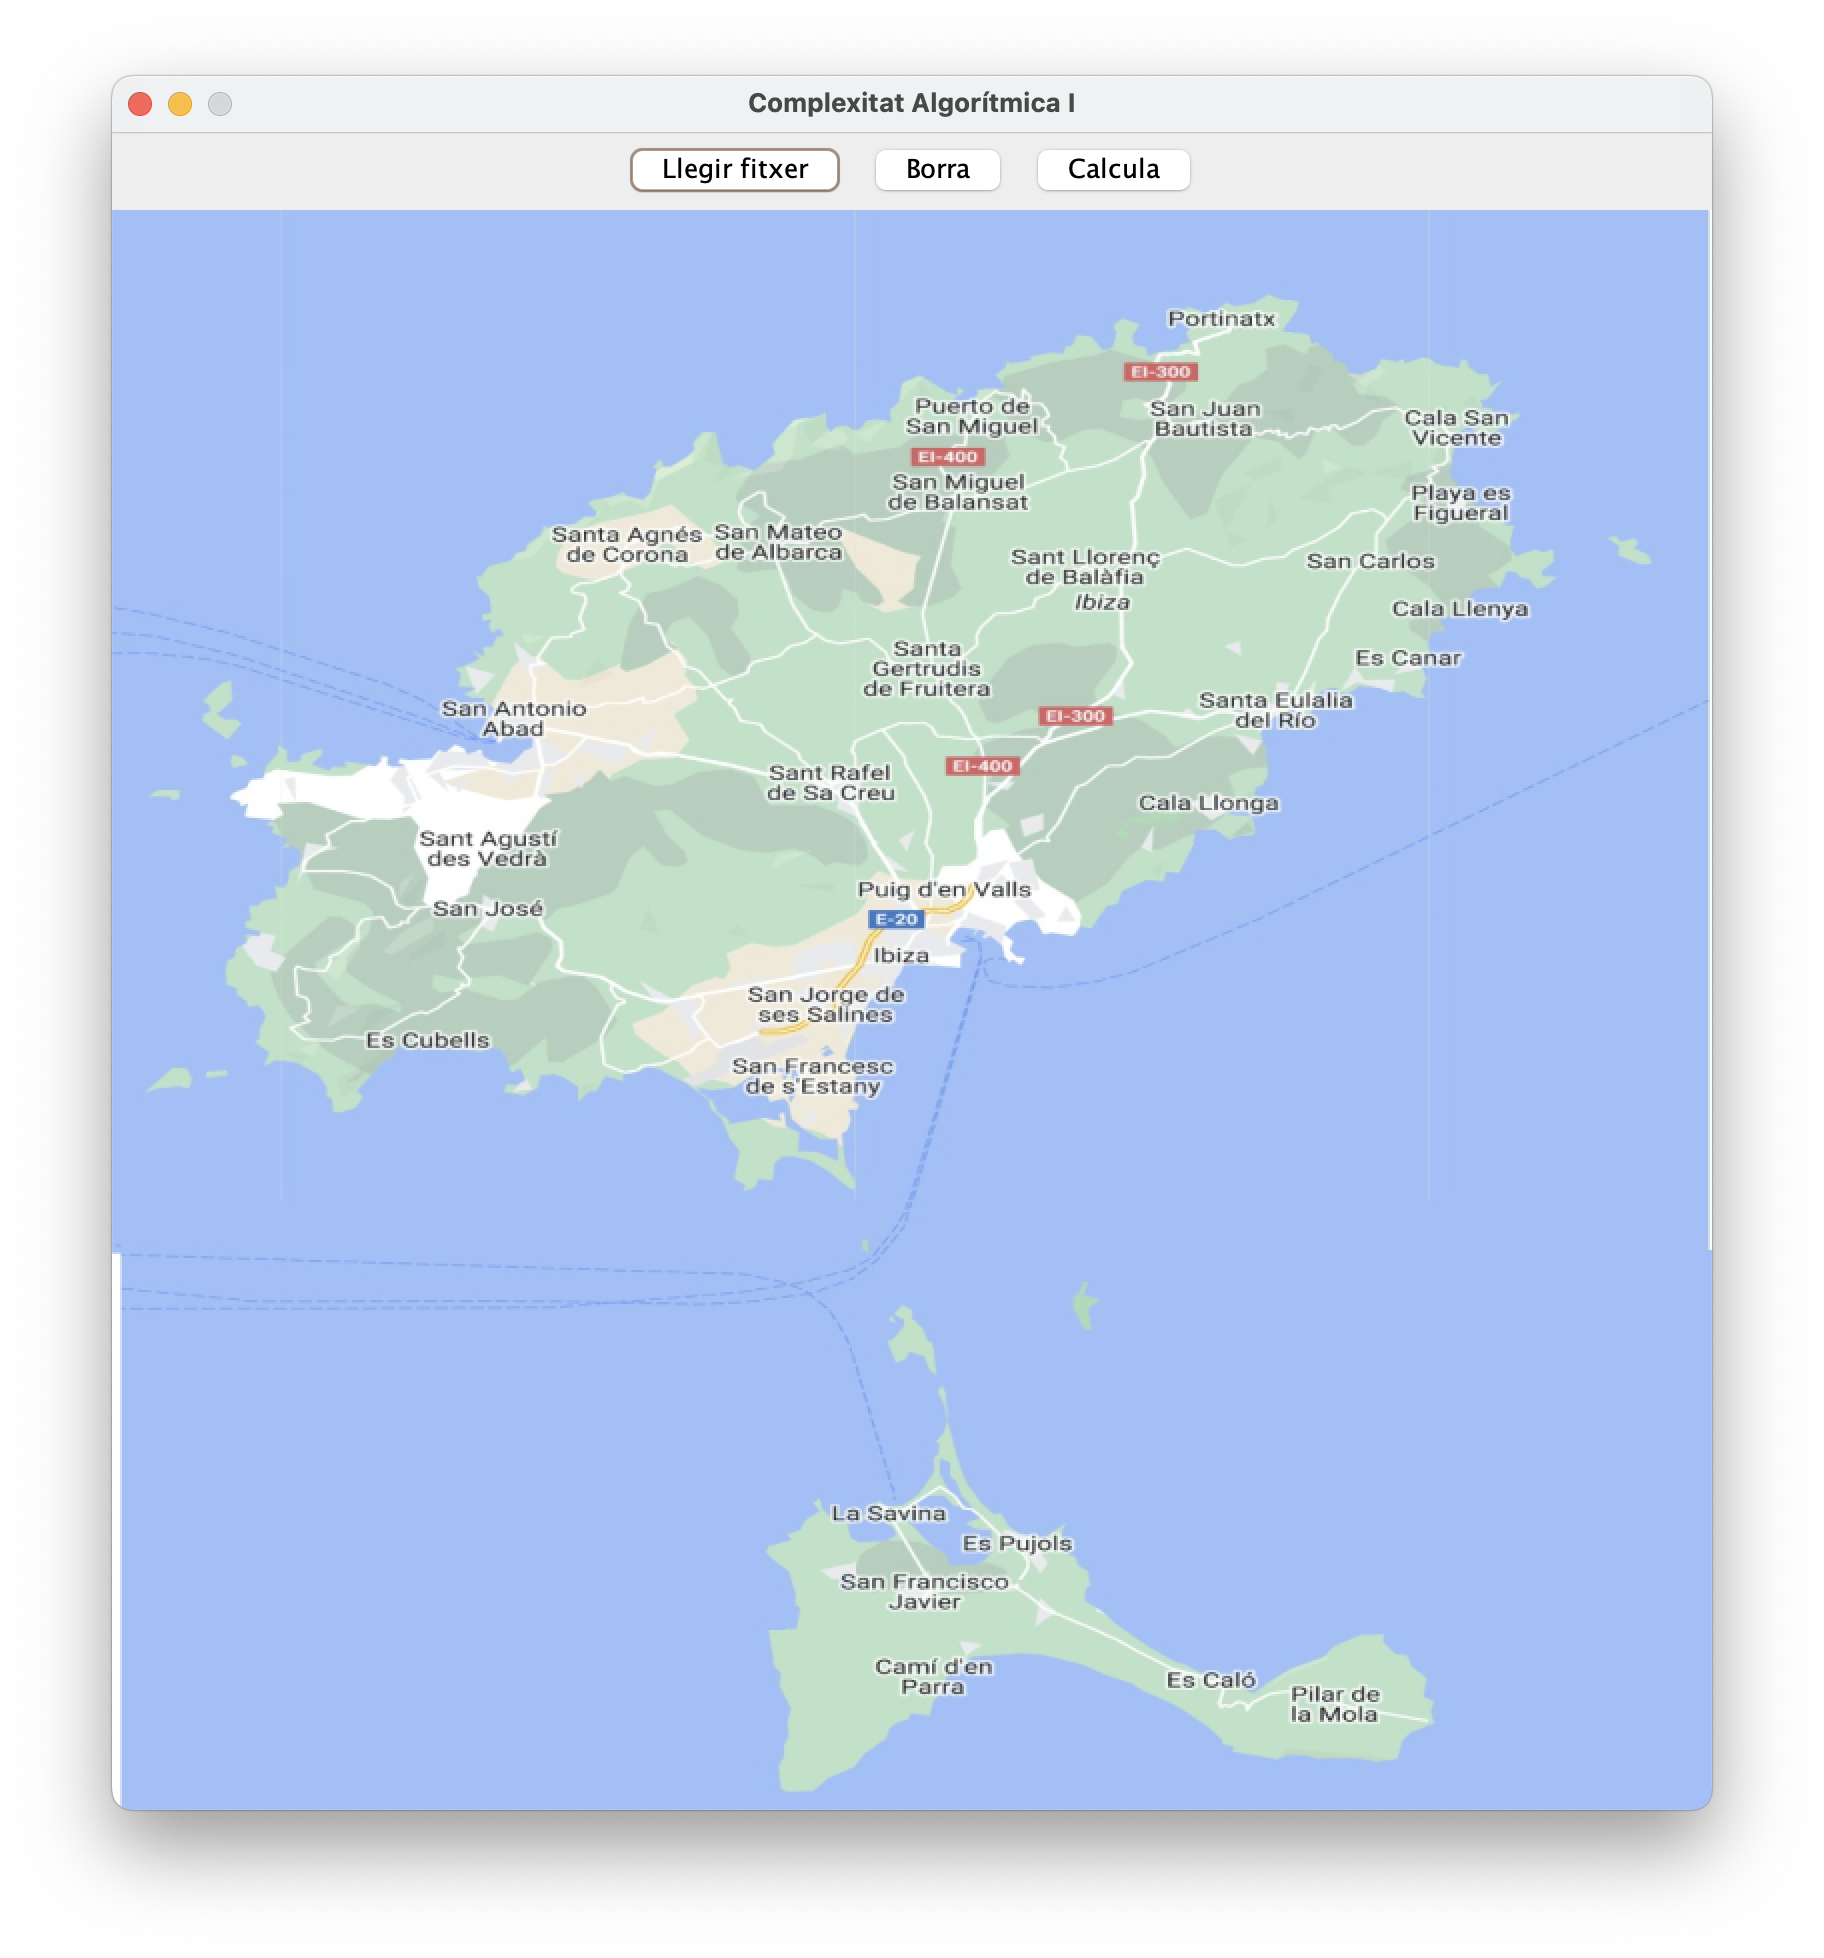
\includegraphics[width=0.388\textwidth]{images/GUI.png}
    \caption{Vista general de la nostra GUI}
\end{figure}

%CONTROLADOR
\section{Controlador}
El controlador és l'encarregat de rebre l'instruccio  del programa principal i posar en funcionament la classe Nuvol explicada en apartats anteriors. Depenent de la comanda d'entrada, s'executara un o un altre mètode de la classe. Els atributs de la classe són els següents:

\begin{verbatim}
private final ibizaDjikstra prog;
private String msg;
private Dijkstra d;
\end{verbatim}

\begin{itemize}
    \item \texttt{prog}: es tracta de una instancia del programa principal la qual utilitzarem per obtenir les dades que es troben al model de dades.\\
    \item \texttt{msg}: variable de tipus \texttt{String} que conté el missatge que rep el mètode \texttt{notifica()} del Controlador.\\
    \item \texttt{d}: instancia de la classe \texttt{Dijkstra} que ens serveix per començar a executar el calculs referents a trobar el camí mínim segons les dades que hi hagin introduïdes en aquell moment en el Model.\\
\end{itemize}

Pel que fa als mètodes del Controlador, tenim els següents:

\begin{verbatim}
public Control(ibizaDjikstra p);
public void run();
public void notificar(String s);
\end{verbatim}

\begin{itemize}
    \item \texttt{Control()}: mètode constructor de la classe amb el qual instanciam l'atribut del programa princiapal i inicialitzam l'objecte de la classe Dijkstra.\\
    \item \texttt{run()}: mètode que s'executa quan es crida al mètode \texttt{start()}. Aquest, actua en conceqüencia quan li arriba l'string amb la paraula \textit{Calcula}. En aquest cas, voldrà dir que l'usuari ha carregat el contingut del XML i ha seleccionat els 3 pobles amb els quals executar l'algorisme. D'aquesta forma, executarà el mètode \texttt{trobarPesos()} de la classe Dijkstra i modificarà les dades del model mitjançant aquest.\\
    \item \texttt{notificar()}: mètode que simplement inicialitza l'atribut \texttt{msg} amb l'string que rep per paràmetre i posa en marxa el mètode \texttt{run()}.\\
\end{itemize}
\section{Programa Principal}
    En aquesta secció s'explicarà la estructura que segueix el nostre programa principal, a més de les accions a realitzar. El nostre programa principal conté com a atributs tres diferents instàncies que implementen el MVC:
\begin{verbatim}
private Model mod;
private Vista vis;
private Control con;
\end{verbatim}
    Amb aquests punters podem accedir a l'informació del model i notificar el diferents events enregistrats. En quant als métodes, el més important i l'únic digne d'explicació es el de \texttt{notificar(String s)} Aquest métode implementa les accions que deriven de l'String rebut per paràmetre, cada posibilitat del switch que utilitzam representa un dels botons de l'interfície les diferentes opcions són:
    \begin{itemize}
        \item \texttt{case 'Llegir fitxer':} : aquest botó s'encarrega de carregar el fitxer i mostrar el graf pertinent. per fer aixó feim servir una instància de la clase \texttt{sax}, aquesta classe li pasam per paràmetre el fitxer i cridam al métode llegir(), vist a classe. Una vegada fet aixó notificam a la vista que ja hem llegit el fitxer.\\
        \item \texttt{case 'Borra':} , aqui reseteam el model i notificam a la vista per a que borri tot el que havia pintat.\\
        \item \texttt{case 'Calcula':} , en aquest botó notificam al control per a que calculi amb el parametre indicat.\\
    \end{itemize}

%JOCS DE PROVES
\section{Joc de proves}
    En aquesta secció ens encarregarem de realitzar 2 jocs de proves diferents, per a comprovar el correcte funcionament de l'aplicació. Aquests testeigs consistiran en escollir 3 diferents pobles per a analitzar les possibles rutes i veure si és la mínima. Cal remarcar, com hem dit anteriorment, que si es passa per un poble més d'un cop, apareix l'ordre dels nombres concatenat amb el caràcter ',' coma.
    \subsection{Primer cas de prova}
    En aquest cas de prova, calcularem la ruta entre aquests 3 pobles:
    $$ruta=\{x_{0}\rightarrow x_{1}\rightarrow x_{2}\}$$
    $$x_{0}\gets \textrm{Cala Llenya}$$
    $$x_{1}\gets \textrm{St Antoni Abad}$$
    $$x_{2}\gets \textrm{La Savina}$$

    \begin{figure}[ht]
        \centering
        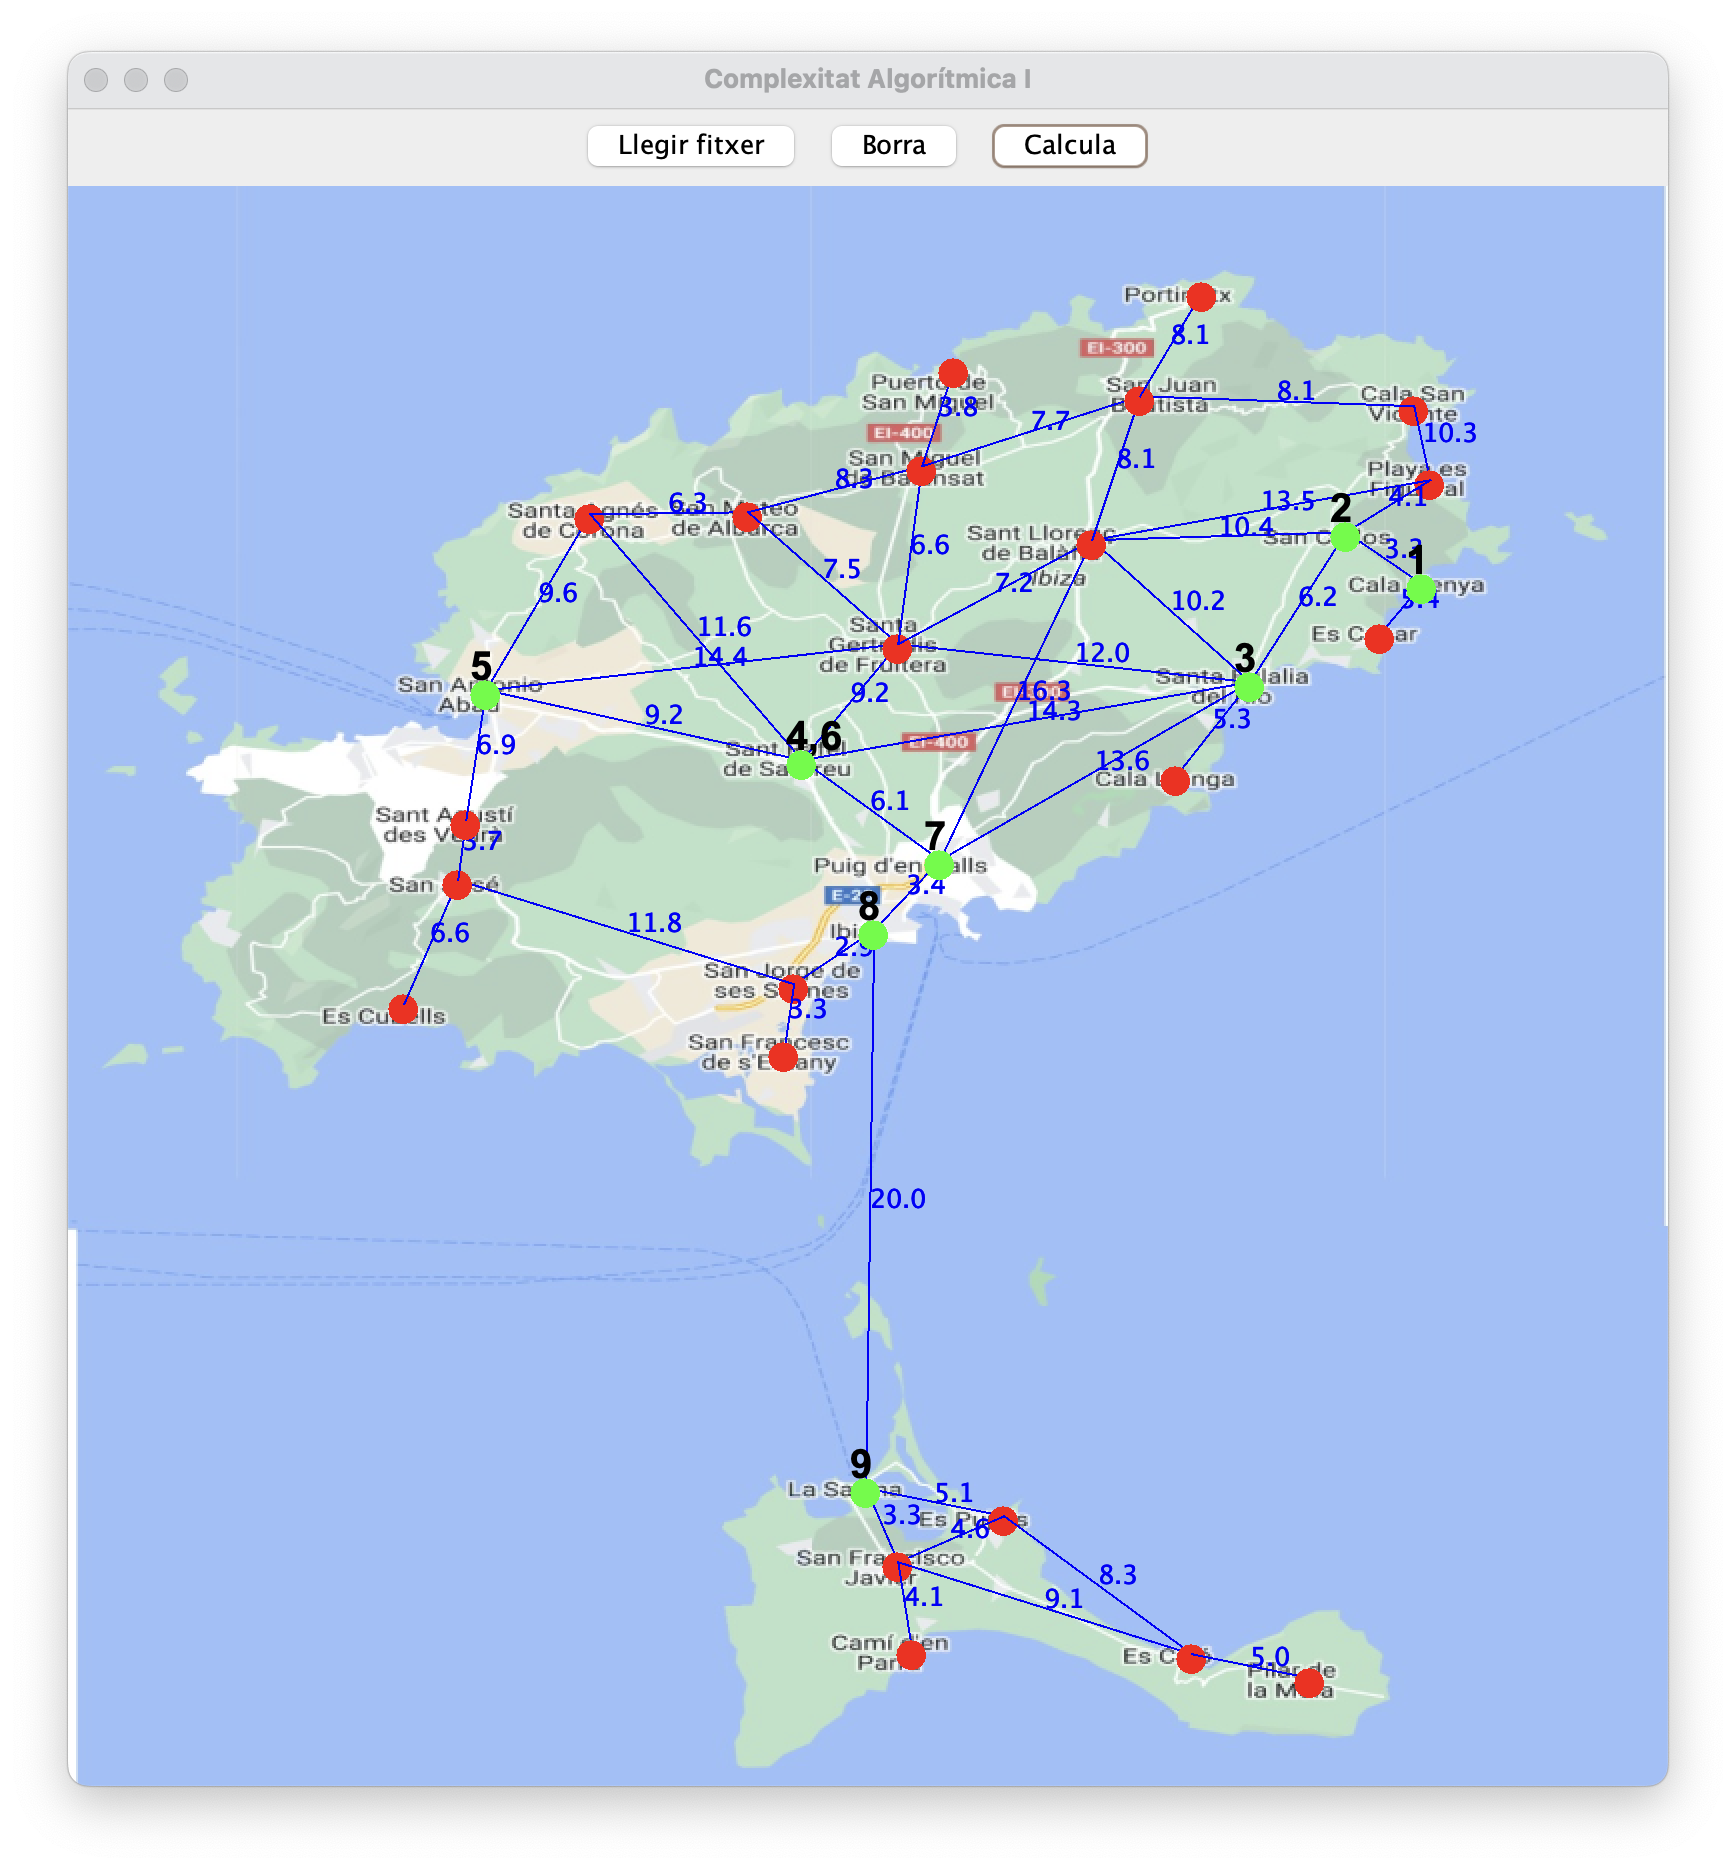
\includegraphics[width=0.4\textwidth]{images/cami_1.png}
        \caption{Recorregut del primer cas de prova}
    \end{figure}

    Com es pot apreciar en la imatge, seguim aquesta ruta:\\\\
    $\textrm{Cala Llenya} \rightarrow \textrm{Sant Carlos} \rightarrow \textrm{Santa Eulàlia del Riu} \rightarrow \textrm{Santa Rafel de Sa Creu} \rightarrow \textrm{Sant Antoni Abad} \rightarrow \textrm{Sant Rafel de Sa Creu} \rightarrow \textrm{Puig d'en Valls} \rightarrow \textrm{Ibiza} \rightarrow \textrm{La Savina}$\\\\
    El cost de la ruta és el següent:

    \begin{figure}[ht]
        \centering
        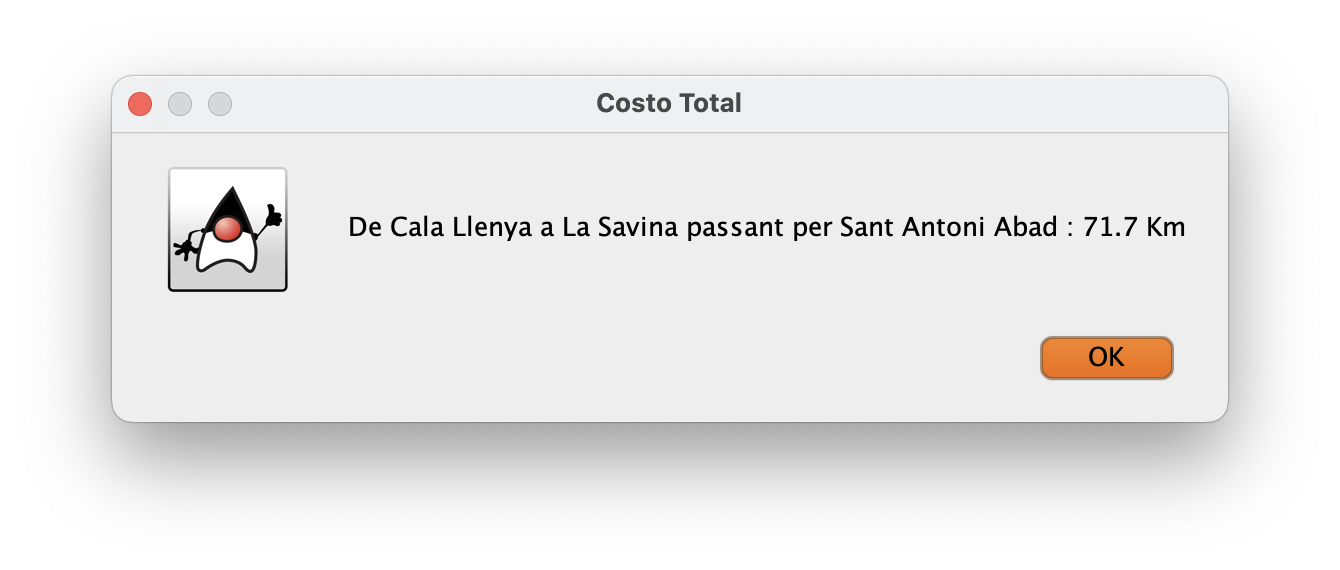
\includegraphics[width=0.388\textwidth]{images/cost1.png}
        \caption{Cost del primer cas de prova}
    \end{figure}

    \subsection{Segon cas de prova}

     En aquest cas de prova, calcularem la ruta entre aquests 3 pobles:
    $$ruta=\{x_{0}\rightarrow x_{1}\rightarrow x_{2}\}$$\\
    $$x_{0}\gets \textrm{Santa Gertrudis de Fruitera}$$
    $$x_{1}\gets \textrm{St Francesc Xavier}$$
    $$x_{2}\gets \textrm{Pilar de la Mola}$$

    \begin{figure}[ht]
        \centering
        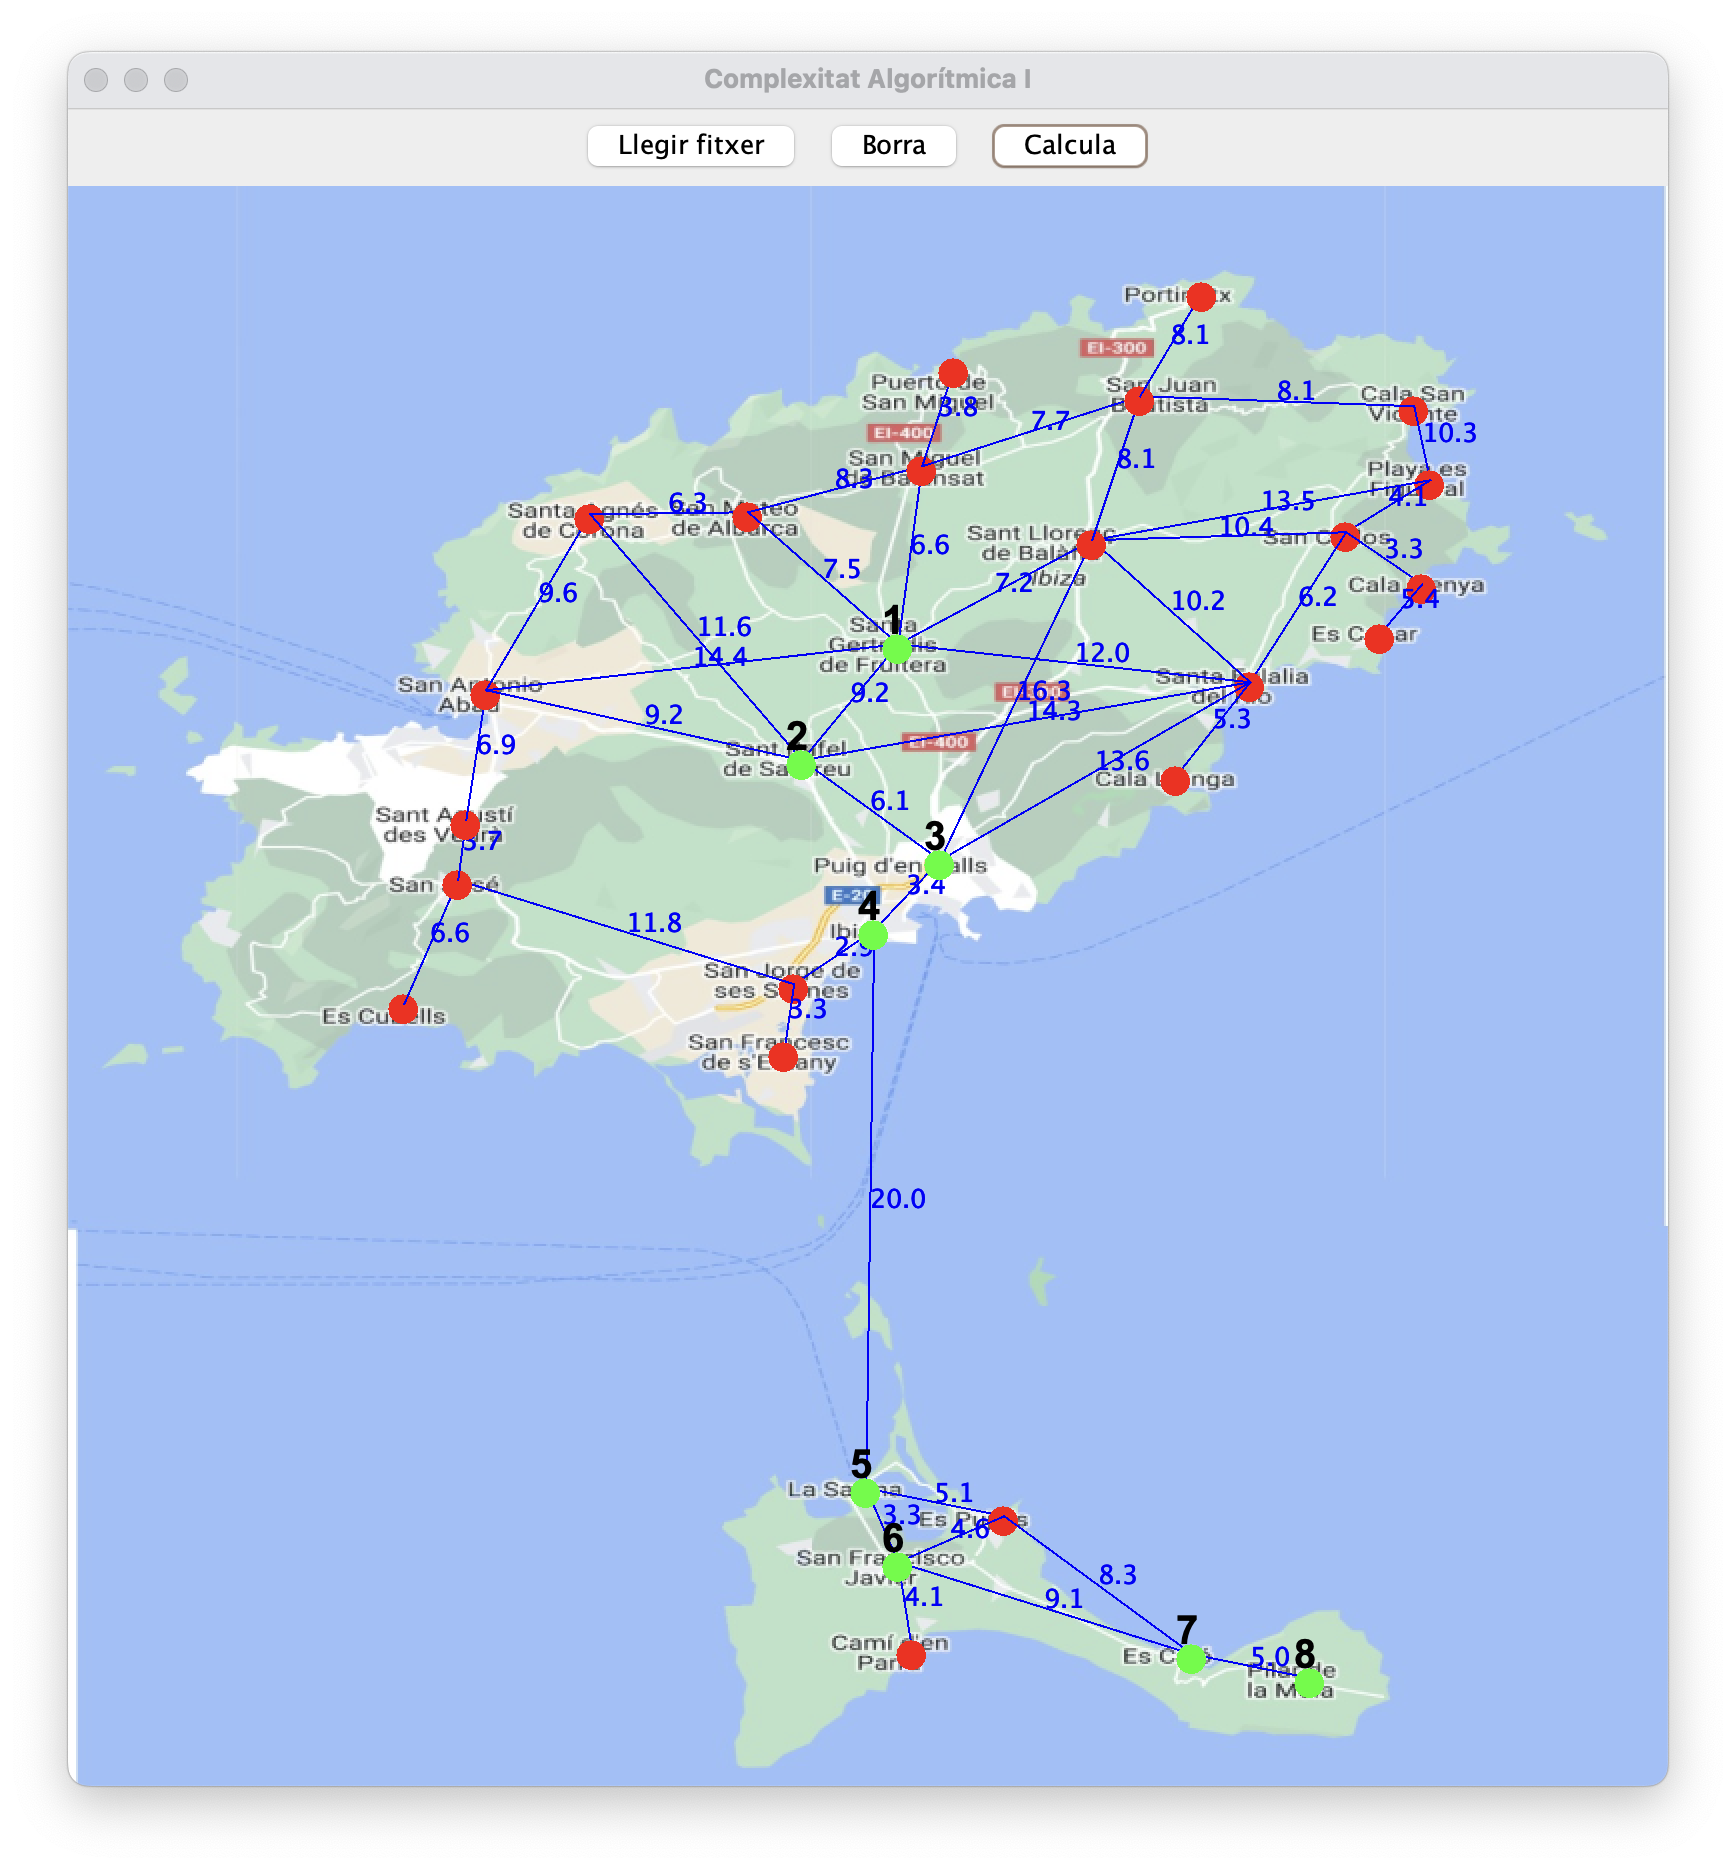
\includegraphics[width=0.4\textwidth]{images/cami_2.png}
        \caption{Recorregut del segon cas de prova}
    \end{figure}

    Com es pot apreciar en la imatge, seguim aquesta ruta:\\\\
    $\textrm{Santa Gertrudis de Fruitera} \rightarrow \textrm{Sant Rafel de Sa Creu} \rightarrow \textrm{Puig d'en Valls} \rightarrow \textrm{Ibiza} \rightarrow \textrm{La Savina} \rightarrow \textrm{Sant Francesc Xavier}\rightarrow \textrm{Puig d'en Valls} \rightarrow \textrm{Ibiza} \rightarrow \textrm{La Savina} \rightarrow \textrm{Sant Francesc Xavier} \rightarrow \textrm{Es Caló} \rightarrow \textrm{Pilar de la Mola}$\\\\
    El cost de la ruta és el següent:
    \begin{figure}[ht]
        \centering
        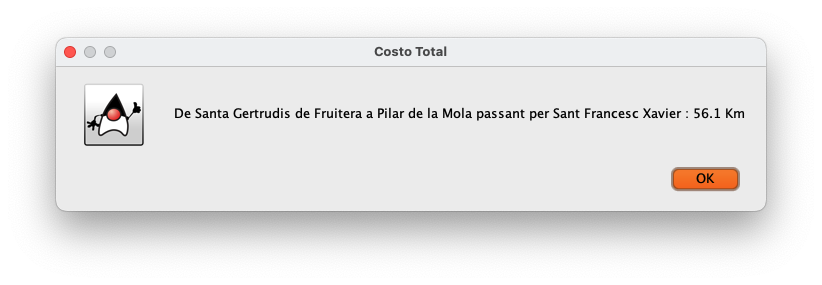
\includegraphics[width=0.388\textwidth]{images/cost_2.png}
        \caption{Cost del segon cas de prova}
    \end{figure}

    \subsection{Tercer cas de prova}
    En aquest cas de prova, calcularem la ruta entre aquests 3 pobles:\\\\
    $$ruta=\{x_{0}\rightarrow x_{1}\rightarrow x_{2}\}$$
    $$x_{0}\gets \textrm{Santa Agnés de Corona}$$
    $$x_{1}\gets \textrm{San José}$$
    $$x_{2}\gets \textrm{Camí den Parra}$$

    \begin{figure}[ht]
        \centering
        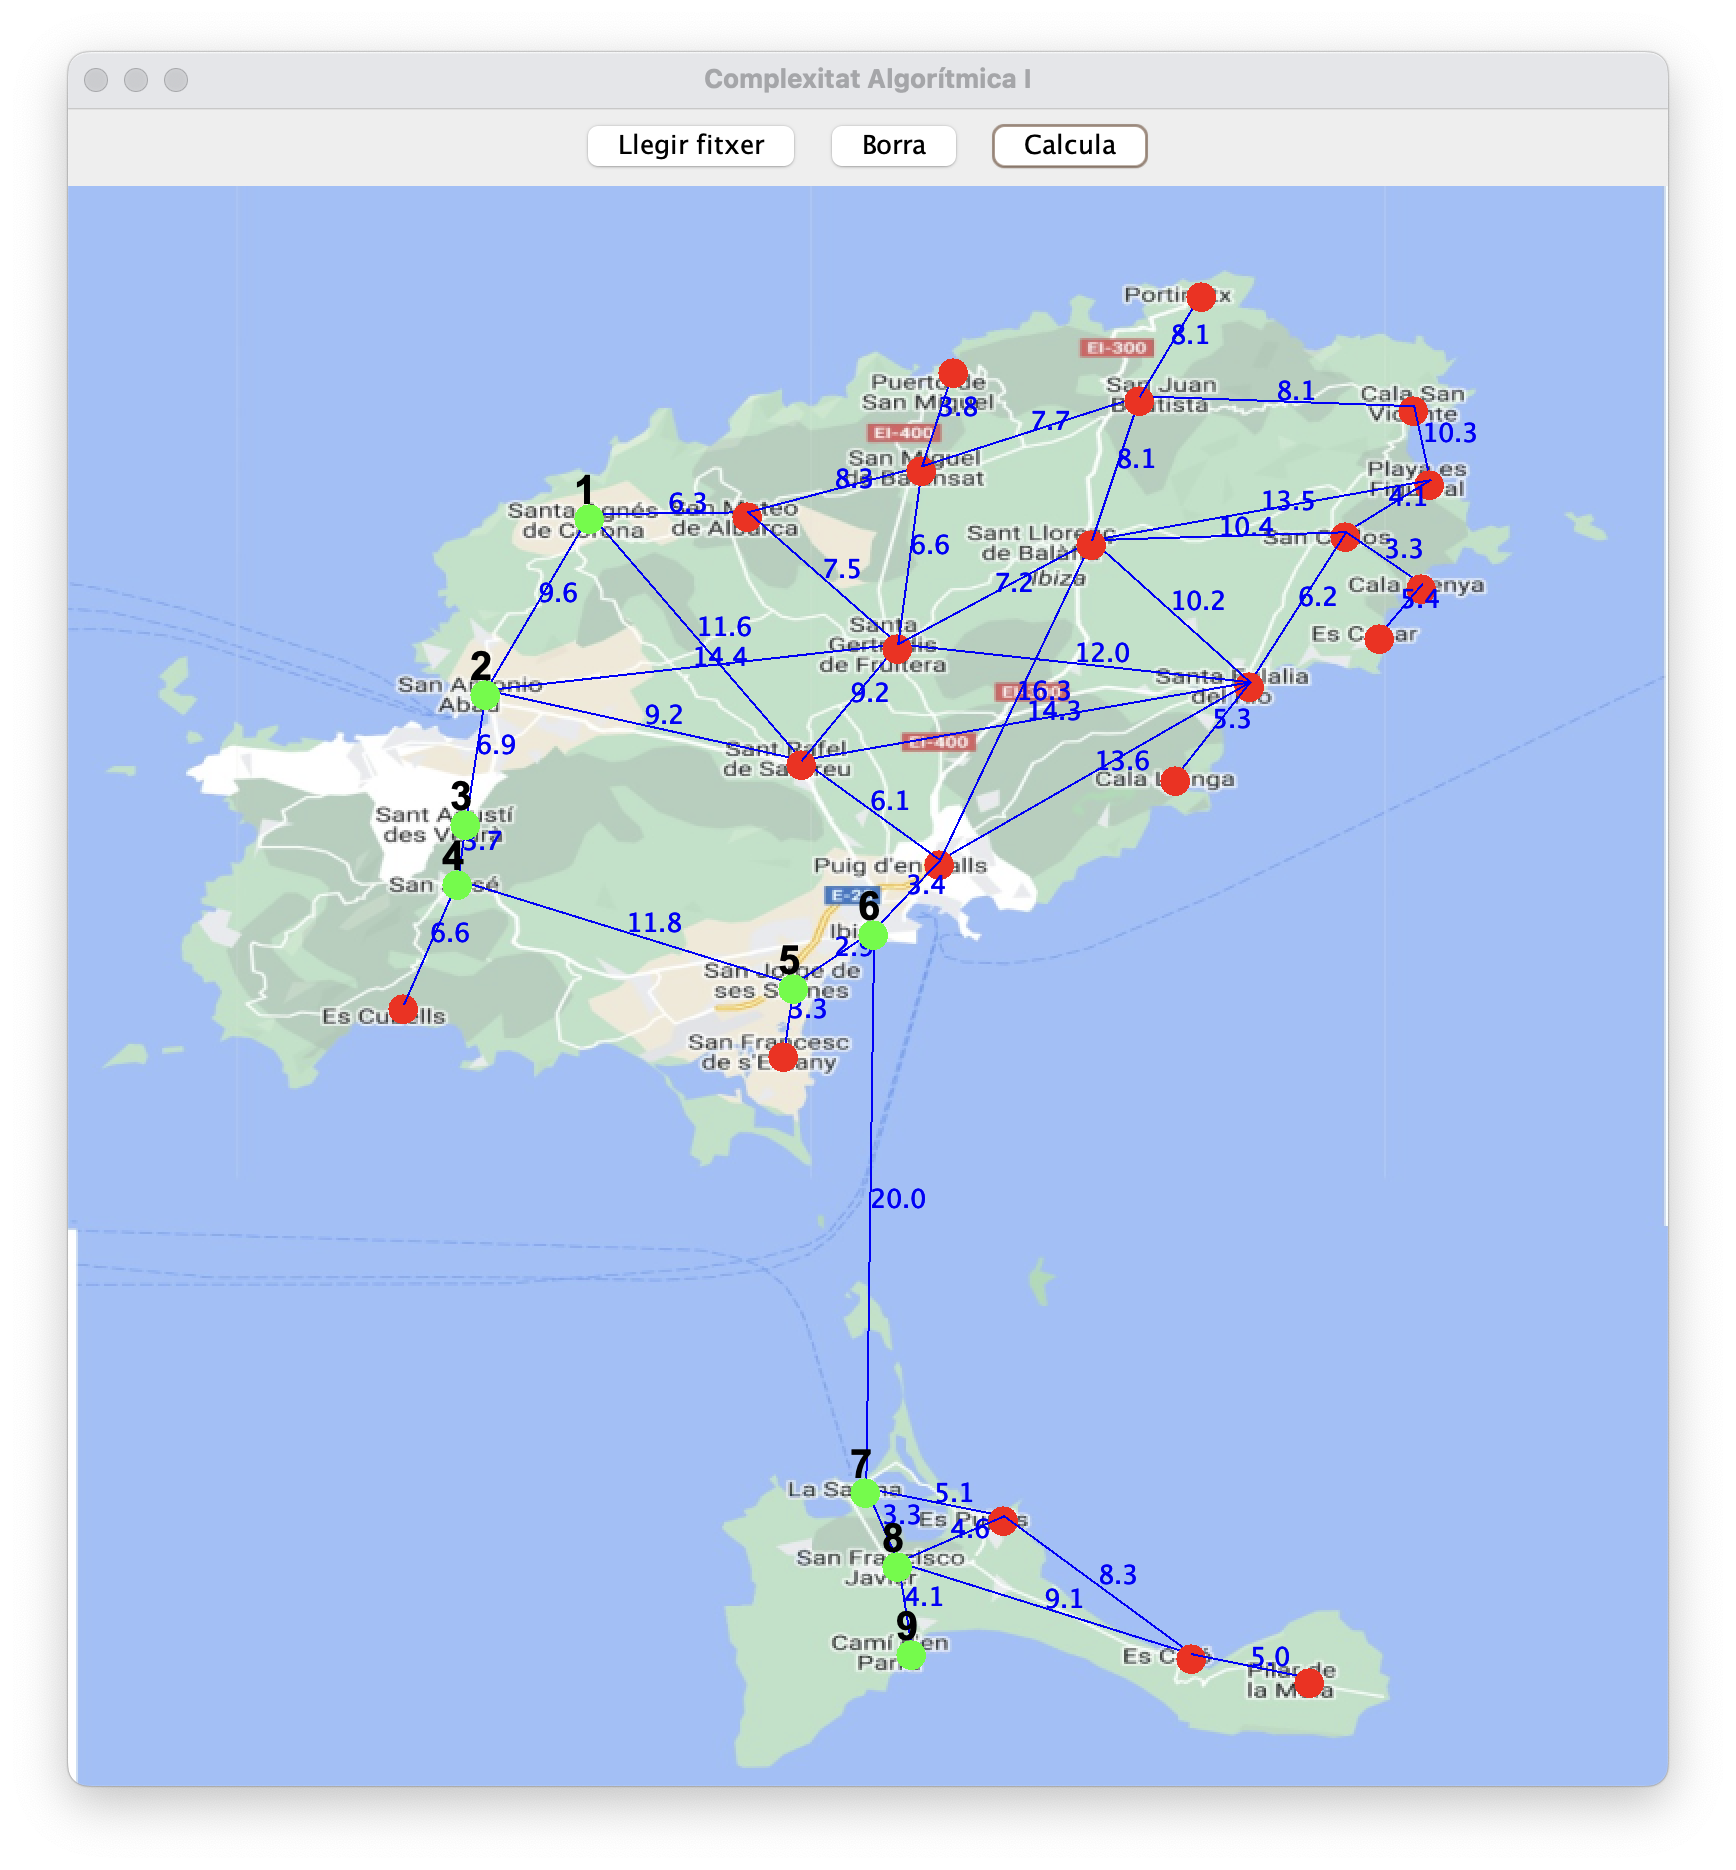
\includegraphics[width=0.4\textwidth]{images/cami_3.png}
        \caption{Recorregut del cost cas de prova}
    \end{figure}

    Com es pot apreciar en la imatge, seguim aquesta ruta:\\\\
    $\textrm{Santa Agnés de Corona} \rightarrow \textrm{Sant Antoni Abad} \rightarrow \textrm{San Agustí des Vedrà} \rightarrow \textrm{San José} \rightarrow \textrm{San Jordi de ses Salines} \rightarrow \textrm{Ibiza}\rightarrow \textrm{La Savina} \rightarrow \textrm{Camí den Parra}$\\\\
    El cost de la ruta és el següent:
    \begin{figure}[ht]
        \centering
        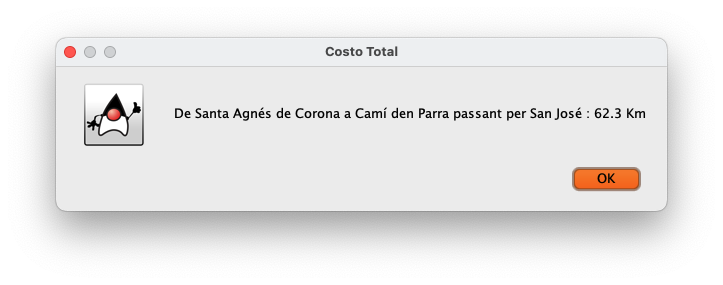
\includegraphics[width=0.388\textwidth]{images/cost_3.png}
        \caption{Cost del tercer cas de prova}
    \end{figure}

\section{Conclusions Finals}
    Aquesta pràctica, tot i no haver comparació de rendiments entre algoritmes, podem extreure unes conclusions finals molt interessants.\\

    En primer lloc, cal destacar que aquesta pràctica compleix el següent principi:\\

    $$\exists S^{*}\quad |\quad S^{*} \in opt$$

    Existeix un conjunt que és òptim, $S^*$, que pertany al grup $opt$, representant la optimalitat.

    $$S^{*}=\{S_{0},S_{1},...S_{n}|\sum_{i=0}^nS_{i}=S^{*}\}$$

    A continuació, podem observar que aquest conjunt és pot dividir en subconjunts més petits $S_i$, de tal manera que afegits tots, formin un altre cop $S^*$. Això vendria a ser com dividir la solució en conjunts més petits.

    $$\forall S_{i} \in S^{*}\rightarrow S_{i} \in opt$$


    Per a qualsevol subconjunt que pertanyi a $S^*$, és demostrat que aquest subconjunt també és òptim. Hem fet la demostració general, però anem a veure el problema des de una perspectiva més enfocada al nostre problema:\\


    $$S^*=\{\textbf{A}\rightarrow\textbf{B}\rightarrow\textbf{C}\}$$

    Suposam que tenim la solució òptima de la ruta que va de \textbf{A} a \textbf{C}, passant per \textbf{B}. Destacam que aquestes tres lletres poden esser 3 pobles qualssevol, no afecta en el principi postulat anteriorment.

    $$S^*=\{S_{0}\cdot S_{1}\quad|\quad S_{0}=\{\textbf{A}\rightarrow\textbf{B}\} \land S_{1}=\{\textbf{B}\rightarrow\textbf{C}\} \}$$

    Com podem apreciar, es pot dividir el problema en anar de \textbf{A} fins a \textbf{B} i després de \textbf{B} fins a \textbf{C}. D'aquesta manera, ambdós subconjunts de la solució són òptims, és a dir, que la solució ve donada per la concatenació dels camins més curts anteriors. \\

    Es pot això complir per a qualsevol ruta que hagui de passar per $n$ pobles?
    Sí i no. Si suposam que enlloc de tenir una ruta amb 3 pobles en tenim entre 4, existeixen dues possibilitats:\\

    $$\exists \textbf{A},\textbf{B},\textbf{C},\textbf{D}$$

    $$S_{0}^*=\{\textbf{A}\rightarrow \textbf{B}\rightarrow \textbf{C}\rightarrow \textbf{D}\}$$

    $$S_{1}^*=\{\textbf{A}\rightarrow \textbf{C}\rightarrow \textbf{B}\rightarrow \textbf{D}\}$$

    Això ens fa pensar en un factor molt important, l'ordre a seguir. El fet de posar aquesta restricció ens fa disminuir el nombre de possibilitats de manera dràstica. Si tenim $n$ pobles i volem fer una ruta del primer al darrer seguint un ordre establert amb els intermigs, podem aplicar el principi anterior. Si és al contrari, ens trobam amb un problema molt més difícil computacionalment. El problema passar a ser del viatjant de comerç.\\

    En aquest cas, quan ens trobam amb el problema del viatjant de comerç, ens estam enfrontant a un problema que pertany a "NP-Hard", que ens diu que no es pot resoldre amb un temps polinomial, sinó que és exponencial. Tot i haver implementacions que arriben a trobar solucions molt pròximes a la òptima, no es garanteix el fet de trobar la solució òptima en temps polinomial. Si no és troba la solució òptima, no garanteix que qualsevol conjunt més petit sigui òptim també.\\

    En conclusió, podem extreure dos idees molt importants:\\


    \begin{itemize}
        \item \textbf{Divisió de solucions òptimes}: el nostre estudi ens ha demostrat que donat qualsevol conjunt $S^*$ amb la solució òptima compleix aquest principi:

        $$\forall S_{i} \in S^*\rightarrow S_{i}\in opt$$

        Per tant, si hem trobat el camí més curt de Palma cap a Sóller passant per Inca,per posar un exemple, haurem trobat dos camins més curts. El primer és el de Palma cap a Inca i l'altre el de Inca cap a Sóller, evitant així possibles càlculs en un futur.\\
        \item \textbf{L'ordre és un factor molt important}: per a qualsevol nombre $n>3$ que tenguem, s'haurà de establir una ruta si volem tenir un problema que es pugui resoldre en temps polinòmic. Remarcam que això comença a passar quan $n=4$.
        
    \end{itemize}




\section{Bibliografia}
\begin{itemize}
    \item \href{https://www.geeksforgeeks.org/dijkstras-shortest-path-algorithm-greedy-algo-7/}{GeeksForGeeks}
    \item \href{https://www.youtube.com/watch?v=quH8JShX33o}{Video Explicatiu de la Pràctica amb execucions}
\end{itemize}
    



\end{document}
